%**********************************************************************%
% _                    _                       _       _
% | |__   ___ _ __ ___ | |_ ___ _ __ ___  _ __ | | __ _| |_ ___
% | '_ \ / _ \ '_ ` _ \| __/ _ \ '_ ` _ \| '_ \| |/ _` | __/ _ \
% | |_) |  __/ | | | | | ||  __/ | | | | | |_) | | (_| | ||  __/
% |_.__/ \___|_| |_| |_|\__\___|_| |_| |_| .__/|_|\__,_|\__\___|
%                                        |_|
%----------------------------------------------------------------------%
\RequirePackage{plautopatch} %日本語パッケージを使う.
\documentclass[aspectratio=169, 12pt]{beamer} %  8pt, 9pt, 10pt, 11pt, 12pt, 14pt, 17pt, 20pt
\usetheme{Madrid}% テーマは指定しなくともよい.
%**********************************************************************%
% フォント
%----------------------------------------------------------------------%
\usepackage{luatexja} %日本語文書の組版を行う
\usepackage[T1]{fontenc} %アクセント記号をUTF-8で使用する.
\usepackage{inconsolata-nerd-font} %等幅フォント consolas
% 和文の既定フォントをゴシックに変更
\renewcommand{\kanjifamilydefault}{\gtdefault}
% Beamerによる数式フォントの置き換えを阻止
\usefonttheme{professionalfonts} 
%**********************************************************************%
% 数
%----------------------------------------------------------------------%
\usepackage{amsmath, amssymb} % 数式パッケージ
\usepackage{mathrsfs} %筆記体 $\mathscr{H}$ $\mathscr{L}$
\usepackage{bm} % for vector
%**********************************************************************%
% 図表
%----------------------------------------------------------------------%
\usepackage{here} %[H]オプション : 図表を文中のその場所に配置
\usepackage{ulem} % for \sout{} 取り消し線
\usepackage{booktabs} % \toprule \midrule \bottomrule
\usepackage{xcolor} %色
\usepackage{comment} %\begin{comment} \end{comment}でコメントアウト
\usepackage{boites} %ボックス内で改ページ可 
\usepackage{here, amsmath, latexsym, amssymb, bm, ascmac, mathtools, multicol, tcolorbox, subfig}

%**********************************************************************%
%      _                                       _
%   __| | ___   ___ _   _ _ __ ___   ___ _ __ | |_
%  / _` |/ _ \ / __| | | | '_ ` _ \ / _ \ '_ \| __|
% | (_| | (_) | (__| |_| | | | | | |  __/ | | | |_
%  \__,_|\___/ \___|\__,_|_| |_| |_|\___|_| |_|\__|
%**********************************************************************%



\begin{document}
%---------------------------------------------------------------
% タイトルスライド
%! 聞き流し数学1
\title{聞き流し数学A}
\author[物理の計算屋]{物理の計算屋}
\date{}
\frame{\maketitle} % タイトルページ
%---------------------------------------------------------------
\begin{frame}{個数定理}
    %! 
    \begin{itemize}
        \item $n(A\cup B) = n(A) +n(B) -n(A\cup B)$ \par
              特に$A\cap B = \varnothing$ のとき $n(A\cup B) = n(A) +n(B)$
        \item $n(\bar{A})=n(U)-n(A)$ (Uは全体集合, Aはその部分集合)
        \item $n(A\cup B \cup C)$ \par
              $= n(A) +n(B) +n(C)-n(A\cap B) -n(B\cap C)-n(C\cap A)+n(A\cap B \cap C)$
    \end{itemize}
\end{frame}
%---------------------------------------------------------------
\begin{frame}{集合の要素の個数の性質}
    %! 
    \begin{itemize}
        \item $n(U) \geq n(A\cup B)$
        \item $n(A\cap B) \leq n(A)$, $n(A\cap B) \leq n(B)$
        \item $n(A\cup B) \leq n(A)+n(B)$
    \end{itemize}
\end{frame}
%---------------------------------------------------------------
\begin{frame}{場合の数の数え方}
    %! 
    辞書式配列法や樹形図を用いてもれなく, 重複することなく数え上げる.
\end{frame}
%---------------------------------------------------------------
\begin{frame}{和の法則, 差の法則}
    %! 
    \begin{itemize}
        \item 和の法則 \par
              事柄$A$, $B$の起こり方がそれぞれ$a$, $b$通りで$A$, $B$が同時に起こらないとき, $A$または$B$のどちらかが起こる場合の数は$a+b$通りである.
        \item 積の法則 \par
              事柄$A$の起こり方が$a$通りあり, その各々に対して事柄$B$の起こり方が$b$とおりあるとすると, $A$と$B$がともに起こる場合の数は$ab$通りである.
    \end{itemize}
\end{frame}
%---------------------------------------------------------------
\begin{frame}{順列}
    %! 
    \begin{center}

        \begin{eqnarray*}
            _nP_r&=&n(n-1)(n-2)\cdots (n-r+1) \\
            &=&\frac{n!}{(n-r)!} \;\;\;\;\;(0\leq r \leq n) \\
            &=&\prod_{i=0}^{r-1} \\
            0! &=& 1 \\
            _nP_n&=&n!
        \end{eqnarray*}
    \end{center}
\end{frame}
%---------------------------------------------------------------
\begin{frame}{円順列}
    %! 
    \begin{eqnarray*}
        \frac{n!}{n}=(n-1)! = \frac{_nP_n}{n}
    \end{eqnarray*}
\end{frame}
%---------------------------------------------------------------
\begin{frame}{じゅず順列}
    %! 
    \begin{eqnarray*}
        \frac{(n-1)!}{2}=\frac{円順列}{2}
    \end{eqnarray*}
\end{frame}
%---------------------------------------------------------------
\begin{frame}{重複順列 $n^r$}
    %! 
    \begin{itemize}
        \item $n$個の異なるものをA, B \space2組に分ける$2^n-2$
        \item A, B 2組に分ける $(2^2-2)/2$
        \item A, B, C\space3組に分ける $3^n-3(2^n-2)-3$
        \item 3組に分ける $\{3^n-3(2^n-2)-3\}/2$
    \end{itemize}
\end{frame}
%---------------------------------------------------------------
\begin{frame}{組合せの数}
    %! 
    \begin{eqnarray*}
        _nC_r&=&\frac{_nP_r}{r!}=\frac{n!}{r!(n-r)!} \;\;\;\;\;(0\leq r \leq n) \\
        _nC_n&=&1
    \end{eqnarray*}
\end{frame}
%---------------------------------------------------------------
\begin{frame}{$_nC_r$の性質}
    %!
    \begin{eqnarray*}
        _nC_r&=& _nC_{n-r} \;\;\;\;\;(0\leq r \leq n) \\
        _nC_r&=&_{n-1}C_{r-1}+_{n-1}C_r \;\;\;\;\;(1\leq r \leq n-1, 2\leq n)
    \end{eqnarray*}
\end{frame}
%---------------------------------------------------------------
\begin{frame}{組分け}
    %! 
    $n$人をA組$p$人, B組$q$人, C組$r$人に分ける.
    \begin{eqnarray*}
        _nC_p\times _{n-p}C_q=\frac{n!}{p!q!(n-p-q)!}
    \end{eqnarray*}
    単に3組に分けるときには注意が必要
    \begin{itemize}
        \item 3組同時なら$\div 3!$
        \item 2組同時なら$\div 2!$
    \end{itemize}
\end{frame}
%---------------------------------------------------------------
\begin{frame}{同じものを含む順列}
    %! 
    \begin{eqnarray*}
        _nC_p\times _{n-p}C_{q}\times _{n-p-q}C_r \times \cdots = \frac{n!}{p!q!r!\cdots}
    \end{eqnarray*}
    ただし,
    \begin{eqnarray*}
        p+q+r+\cdots=n
    \end{eqnarray*}
\end{frame}
%---------------------------------------------------------------
\begin{frame}{重複の組合せの数}
    %! 
    \begin{eqnarray*}
        _nH_r=_{n+r-1}C_r\;\;\;\;\; (n\leq r であってもよい)
    \end{eqnarray*}
\end{frame}
%---------------------------------------------------------------
\begin{frame}{確立の定義}
    %! 
    全事象$U$のどの根元事象も同様に確からしいとき,\par
    事象$A$の起こる確率$P(A)$は
    \begin{eqnarray*}
        P(A)=\frac{n(A)}{n(U)}=\frac{事象Aの起こる場合の数}{起こりうるすべての場合の数}
    \end{eqnarray*}
\end{frame}
%---------------------------------------------------------------
\begin{frame}{基本性質}
    %! 
    \begin{eqnarray*}
        0 \leq &P(A)& \leq 1 \\
        P(\varnothing)&=&0 \\
        P(U)&=&1
    \end{eqnarray*}
\end{frame}

%---------------------------------------------------------------
\begin{frame}{加法定理}
    %! 
    事象$A$, $B$が互いに排反のとき
    \begin{eqnarray*}
        P(A\cup B)=P(A)+P(B)
    \end{eqnarray*}
\end{frame}
%---------------------------------------------------------------
\begin{frame}{余事象の確立}
    %! 
    \begin{eqnarray*}
        P(\bar{A})=1-P(A)
    \end{eqnarray*}
\end{frame}
%---------------------------------------------------------------
\begin{frame}{独立な試行の確率}
    %! 
    2つの独立な試行$S$, $T$において, $S$では事象$A$が起こり, $T$では事象$B$が起こる事象を$C$とすると,
    \begin{eqnarray*}
        P(C)=P(A)P(B)
    \end{eqnarray*}
\end{frame}
%---------------------------------------------------------------
\begin{frame}{反復試行の確立}
    %! 
    1回の試行で事象$A$の起こる確率が$p$であるとする\par
    この試行を$n$回繰り返すとき, 事象$A$がちょうど$r$回起こる確率は
    \begin{eqnarray*}
        _nC_rp^r(1-p)^{n-r}
    \end{eqnarray*}
\end{frame}
%---------------------------------------------------------------
\begin{frame}{条件付き確率}
    %! 
    事象$A$が起こったときに事象$B$が起こる条件付き確率$P_A(B)$は
    \begin{eqnarray*}
        P_A(B)=\frac{n(A\cap B)}{n(A)}=\frac{P(A\cap B)}{P(A)}
    \end{eqnarray*}
\end{frame}
%---------------------------------------------------------------
\begin{frame}{確率の乗法}
    %! 
    \begin{eqnarray*}
        P(A\cap B)=P(A)P_A(B)
    \end{eqnarray*}
\end{frame}
%---------------------------------------------------------------
\begin{frame}{三角形の二等分線と比}
    %! 
    \begin{itemize}
        \item $\triangle $ABCの$\angle $Aの二等分線と辺BCとの交点Pは, 辺BCを$c$\space:\space$b$に内分する.
        \item $b\neq c$である$\triangle $ABCの外角の二等分線と辺BCの延長線との交点Qは辺BCを$c$\space:\space$b$に外分する.
    \end{itemize}
    \begin{figure}[htbp]
        \begin{center}
            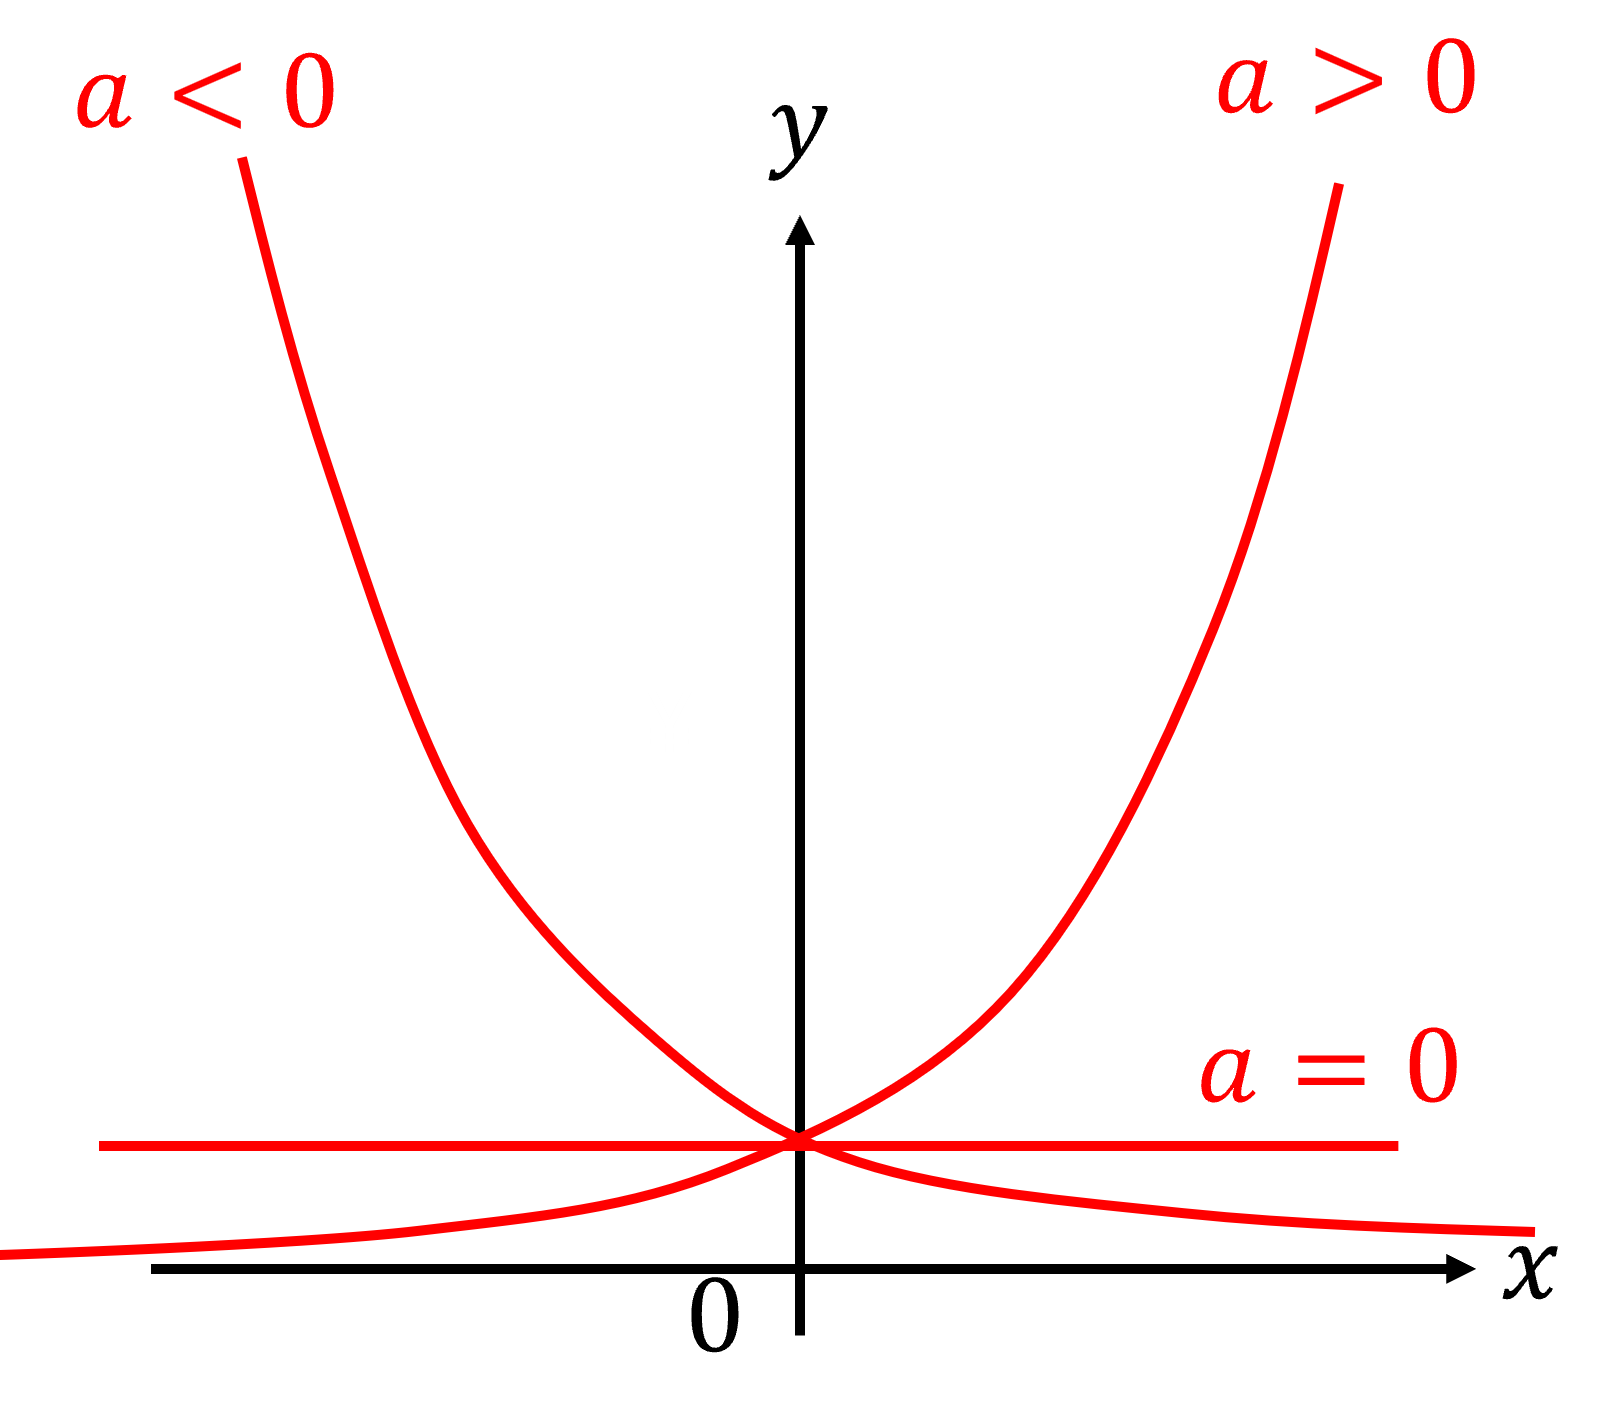
\includegraphics[width=100mm]{fig/1.png}
        \end{center}
    \end{figure}
\end{frame}
%---------------------------------------------------------------
\begin{frame}{外心・内心・重心}
    %! 
    \begin{itemize}
        \item 外心・・・3辺の垂直二等分線の交点
        \item 内心・・・3つの内角の二等分線の交点
        \item 重心・・・3つの中線の交点 \par
              重心は各中点を2\space:\space1に内分する.
        \item 垂心・・・三角形の各頂点から対辺またはその延長に下した垂線の交点
    \end{itemize}
    \begin{figure}[htbp]
        \begin{center}
            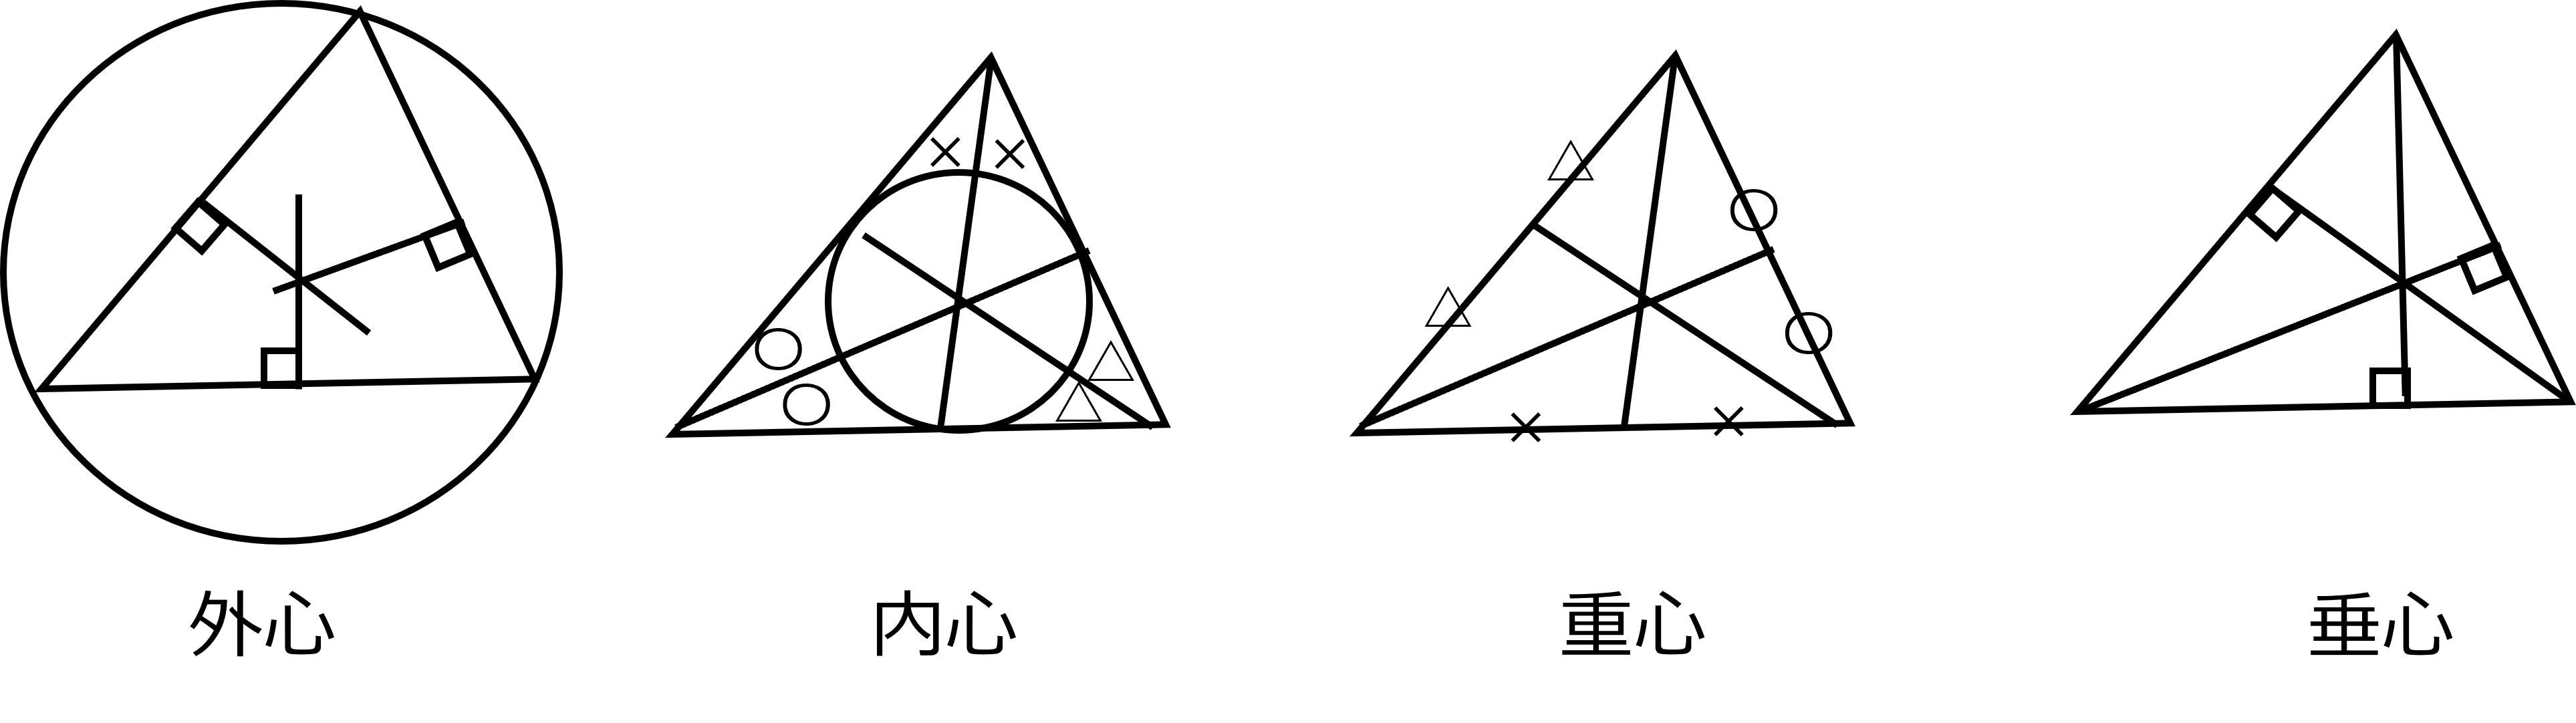
\includegraphics[width=100mm]{fig/2.png}
        \end{center}
    \end{figure}
\end{frame}
%---------------------------------------------------------------
\begin{frame}{チェバの定理}
    %! 
    任意の点O\par
    \begin{eqnarray*}
        \frac{\rm{AR}}{\rm{RB}}\cdot\frac{\rm{BP}}{\rm{PC}}\cdot\frac{\rm{CQ}}{\rm{QA}}=1
    \end{eqnarray*}
    \begin{figure}[htbp]
        \begin{center}
            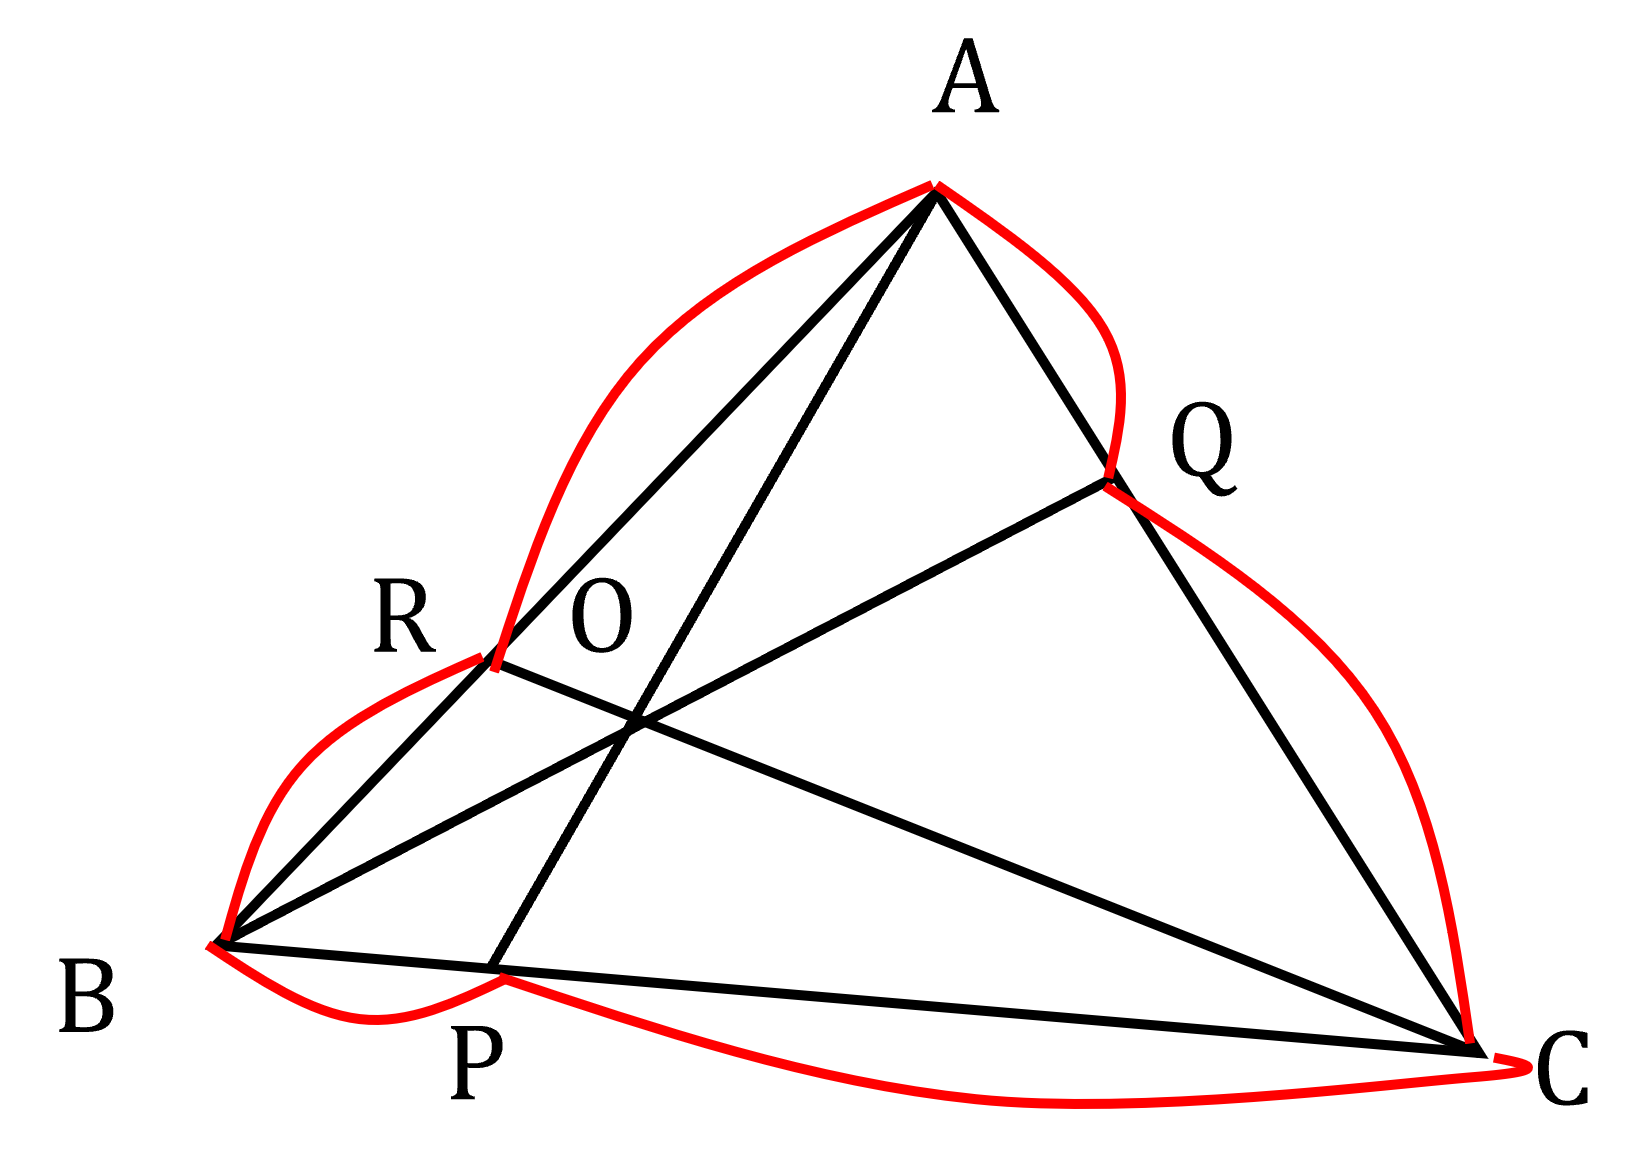
\includegraphics[width=50mm]{fig/3.png}
        \end{center}
    \end{figure}
\end{frame}
%---------------------------------------------------------------
\begin{frame}{メネラウスの定理}
    %! 
    \begin{eqnarray*}
        \frac{\rm{AR}}{\rm{RB}}\cdot\frac{\rm{BP}}{\rm{PC}}\cdot\frac{\rm{CQ}}{\rm{QA}}=1
    \end{eqnarray*}
    \begin{figure}[htbp]
        \begin{center}
            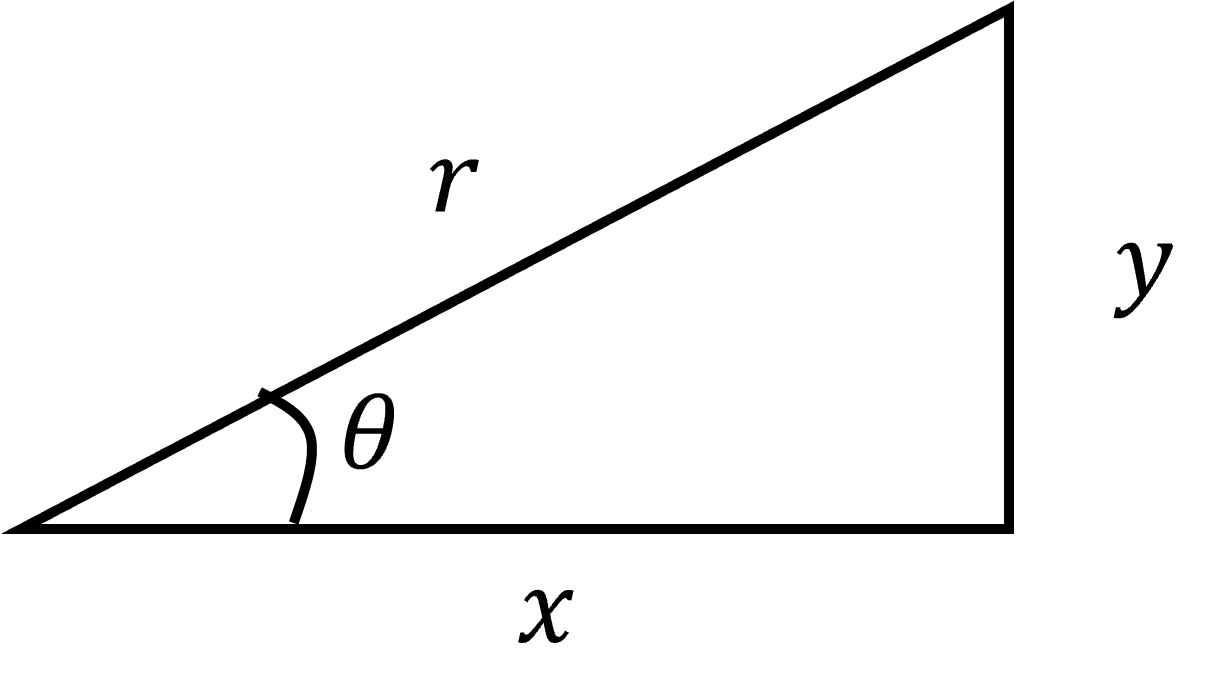
\includegraphics[width=50mm]{fig/4.png}
        \end{center}
    \end{figure}
\end{frame}
%---------------------------------------------------------------
\begin{frame}{円周角の定理とその逆}
    %! 
    \begin{center}
        4点A, B, P, Qが1つの円周上にある.\par
        $\Leftrightarrow \angle $APB$ = \angle $AQB
    \end{center}
    \begin{figure}[htbp]
        \begin{center}
            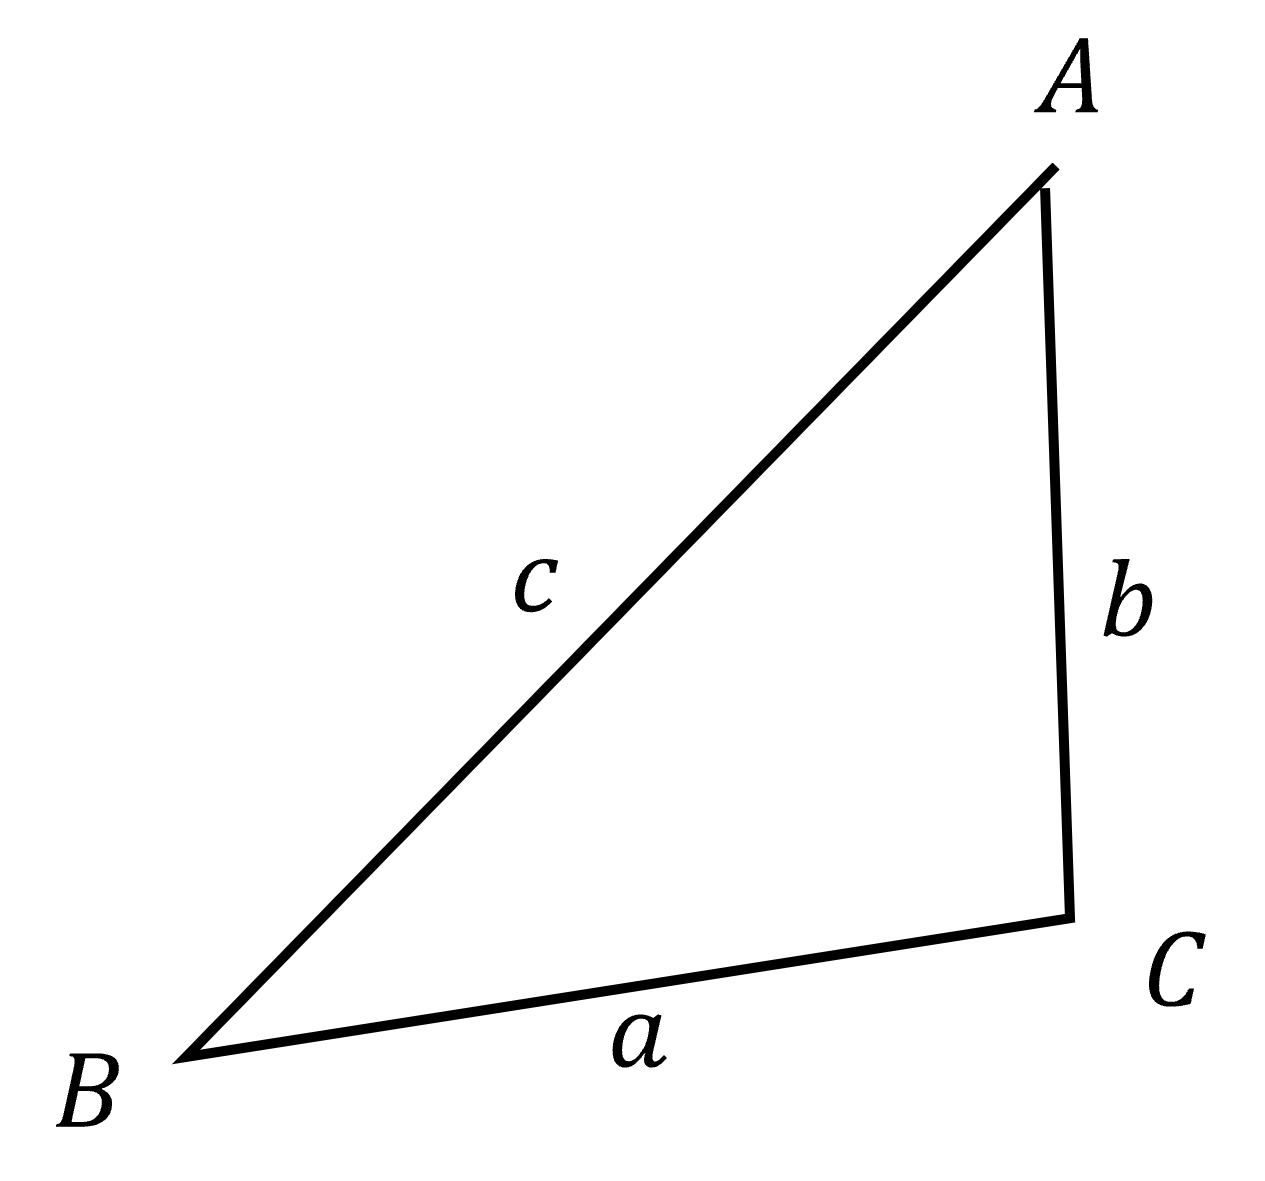
\includegraphics[width=50mm]{fig/5.png}
        \end{center}
    \end{figure}
\end{frame}
%---------------------------------------------------------------
\begin{frame}{円に内接する四角形}
    %! 
    四角形が円に内接するとき次の(1)と(2)が成り立つ.
    \begin{enumerate}
        \item 対角の和は$\pi$
        \item 内角はその対角の外角に等しい
    \end{enumerate}
    \begin{figure}[htbp]
        \begin{center}
            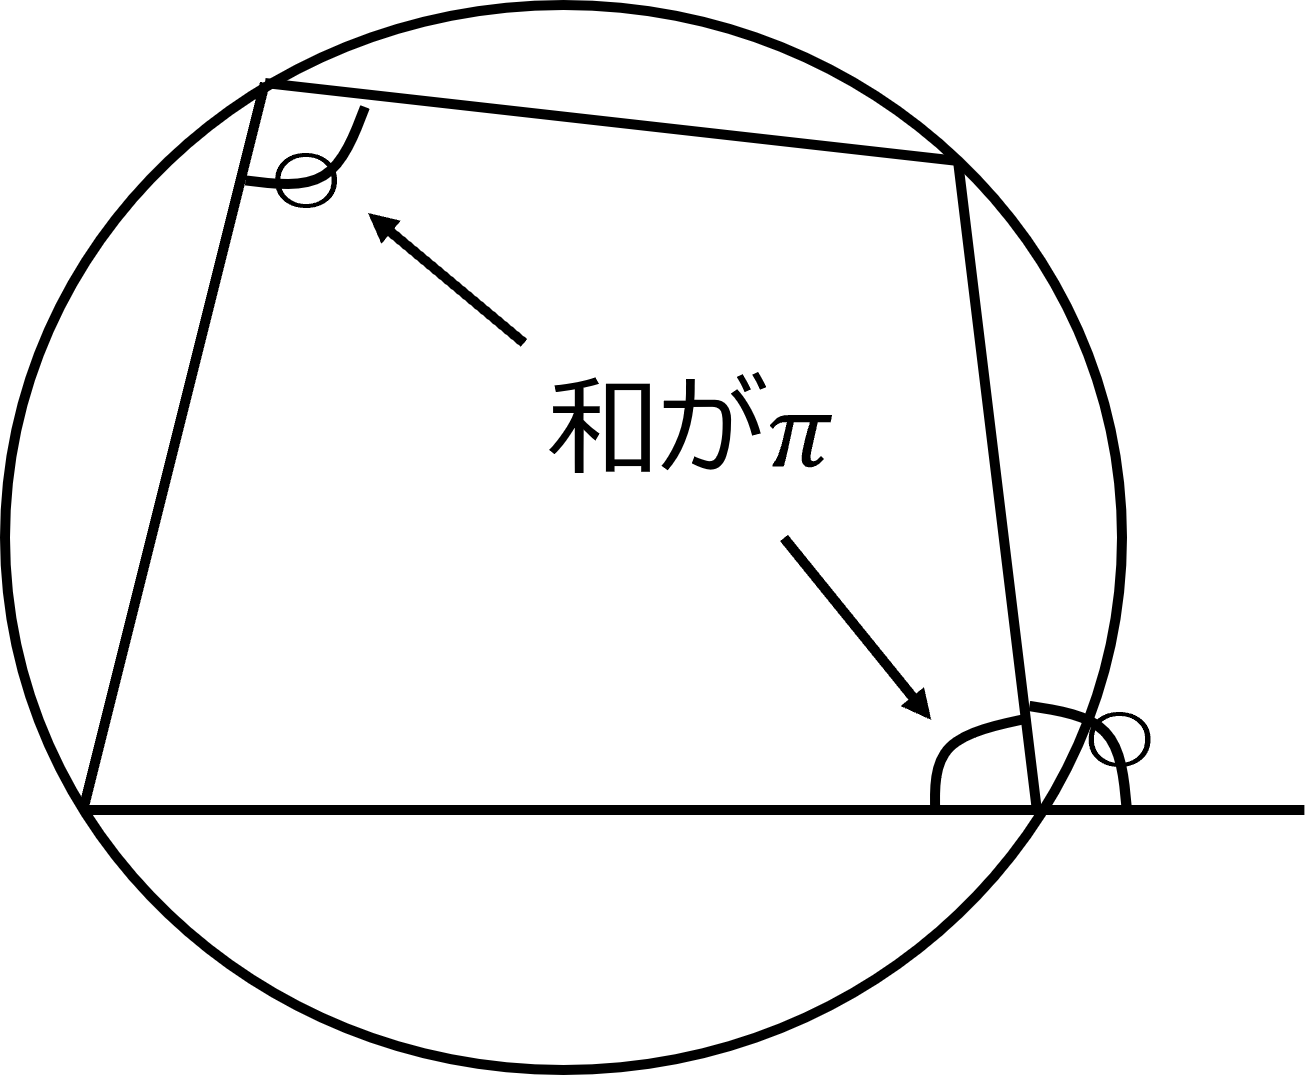
\includegraphics[width=50mm]{fig/6.png}
        \end{center}
    \end{figure}
\end{frame}
%---------------------------------------------------------------
\begin{frame}{円の接線}
    %! 
    \begin{eqnarray*}
        \rm{OA} &\perp& \rm{PA} \\
        \rm{OB} &\perp& \rm{PB} \\
        \rm{PA} &=& \rm{PB}
    \end{eqnarray*}
    \begin{figure}[htbp]
        \begin{center}
            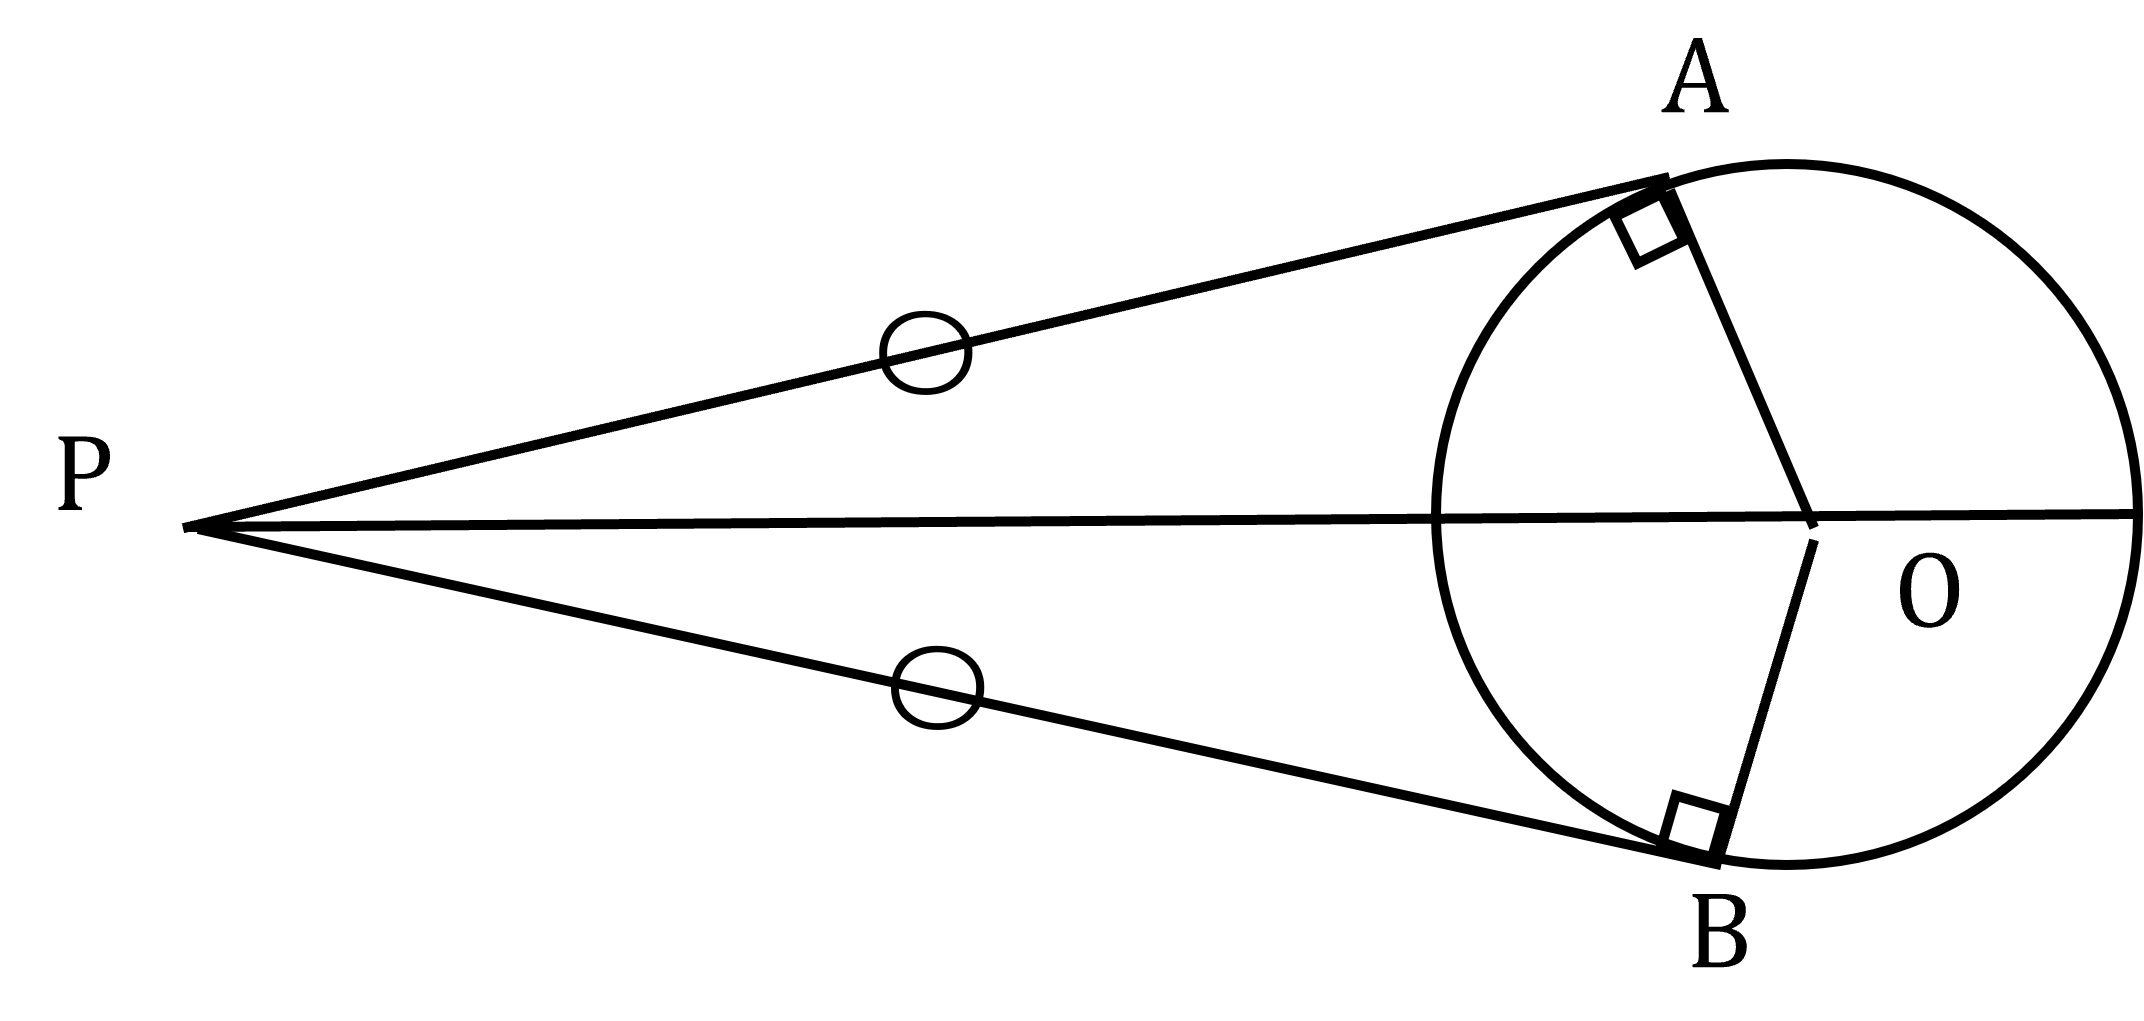
\includegraphics[width=50mm]{fig/7.png}
        \end{center}
    \end{figure}
\end{frame}
%---------------------------------------------------------------
\begin{frame}{接弦定理とその逆}
    %! 
    \begin{center}
        直線ATが円Oの接線
    \end{center}
    \begin{eqnarray*}
        \Leftrightarrow \angle \rm{ACB} = \angle \rm{BAT}
    \end{eqnarray*}
    \begin{figure}[htbp]
        \begin{center}
            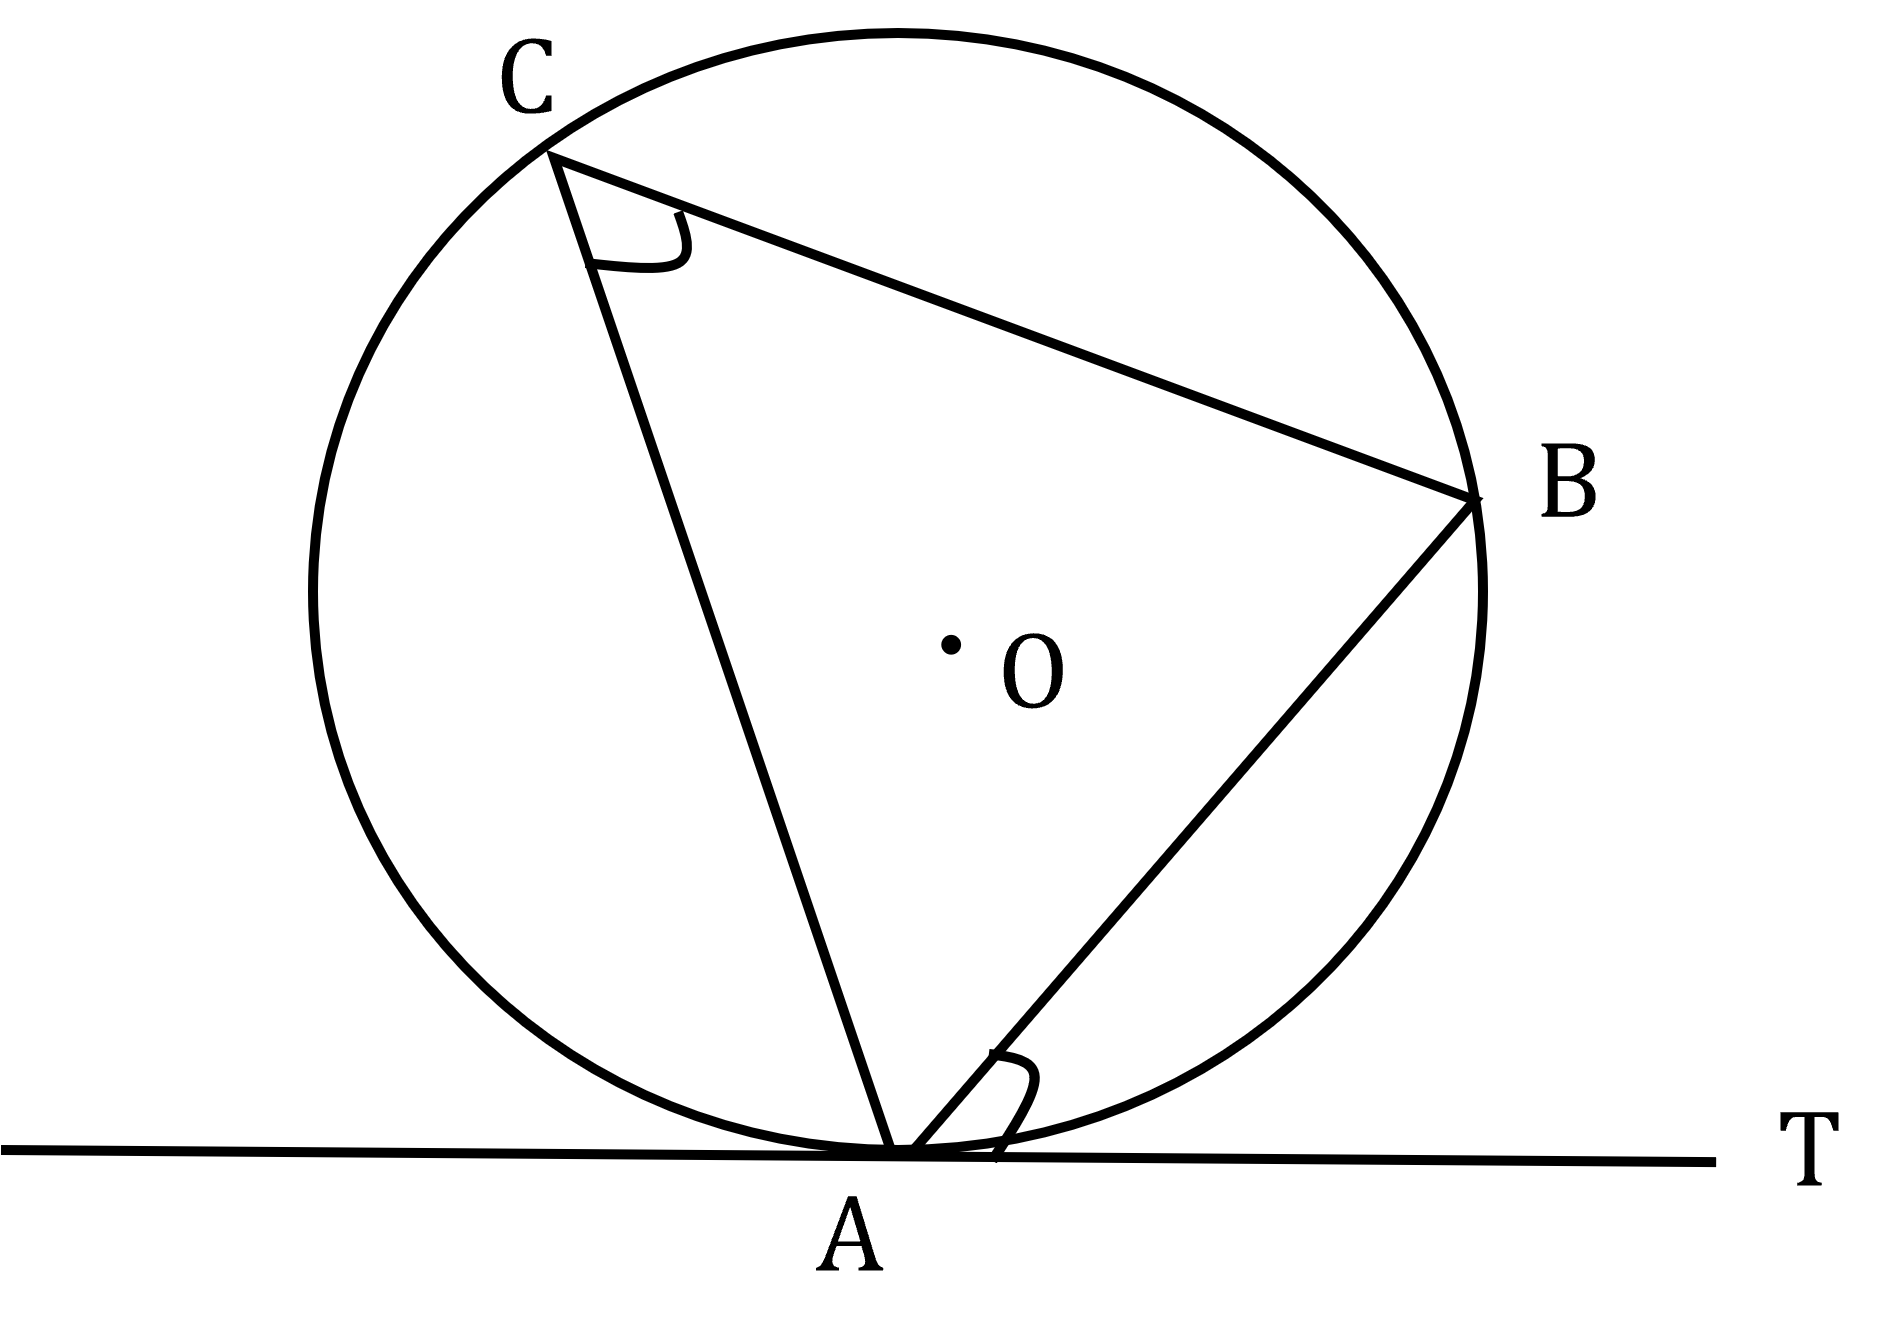
\includegraphics[width=50mm]{fig/8.png}
        \end{center}
    \end{figure}
\end{frame}
%---------------------------------------------------------------
\begin{frame}{方べきの定理 (逆も成り立つ)}
    %! 
    \begin{center}
        $\rm{PA}\cdot \rm{PB} = \rm{PC} \cdot \rm{PD}$, $\rm{PT}^2=\rm{PA}\cdot \rm{PB}$
    \end{center}
    \begin{figure}[htbp]
        \begin{center}
            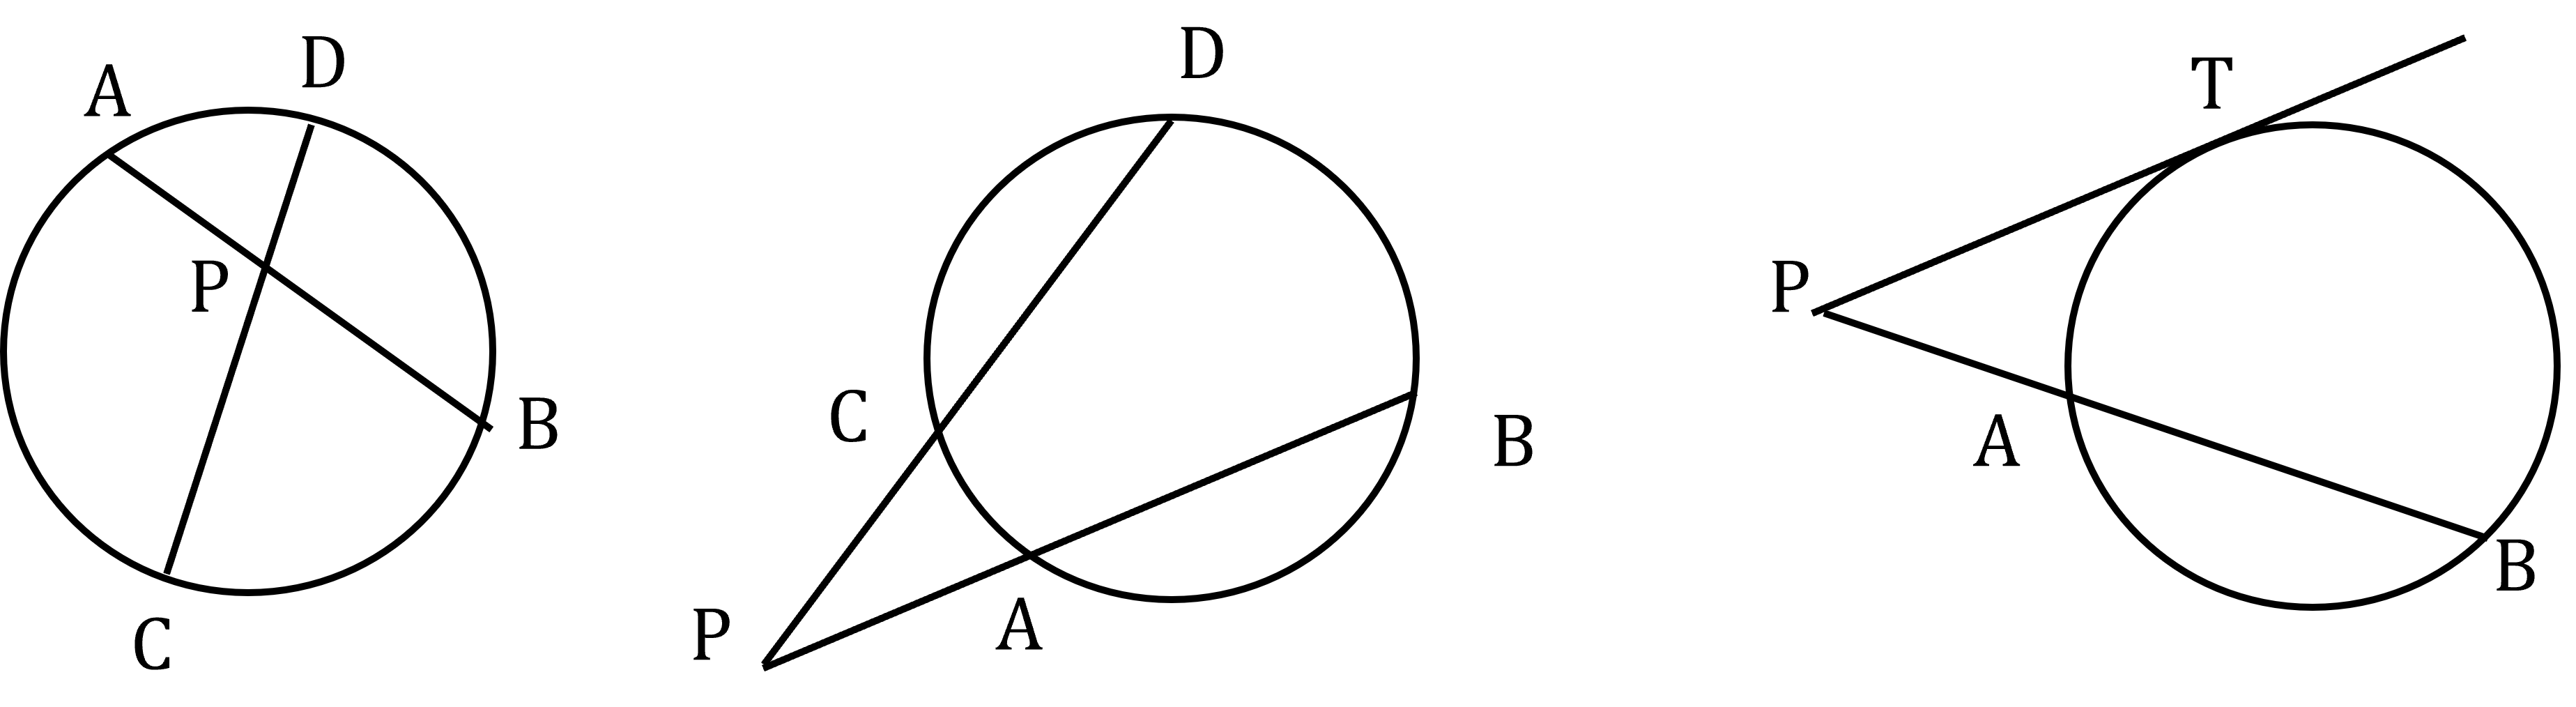
\includegraphics[width=100mm]{fig/9.png}
        \end{center}
    \end{figure}
\end{frame}
%---------------------------------------------------------------
\begin{frame}{三垂線の定理}
    %! 
    平面$\alpha$上に直線$l$があるとき, $\alpha$上にない点A, $l$上の点B, $l$上にない$\alpha$上の点Oについて
    \begin{eqnarray*}
        \rm{AB}\perp l, \;\;\;
        \rm{OB}\perp l, \;\;\;
        \rm{OA}\perp \rm{OB}
    \end{eqnarray*}
    ならば
    \begin{eqnarray*}
        \rm{OA}\perp \alpha
    \end{eqnarray*}
    が成り立つ
    \begin{figure}[htbp]
        \begin{center}
            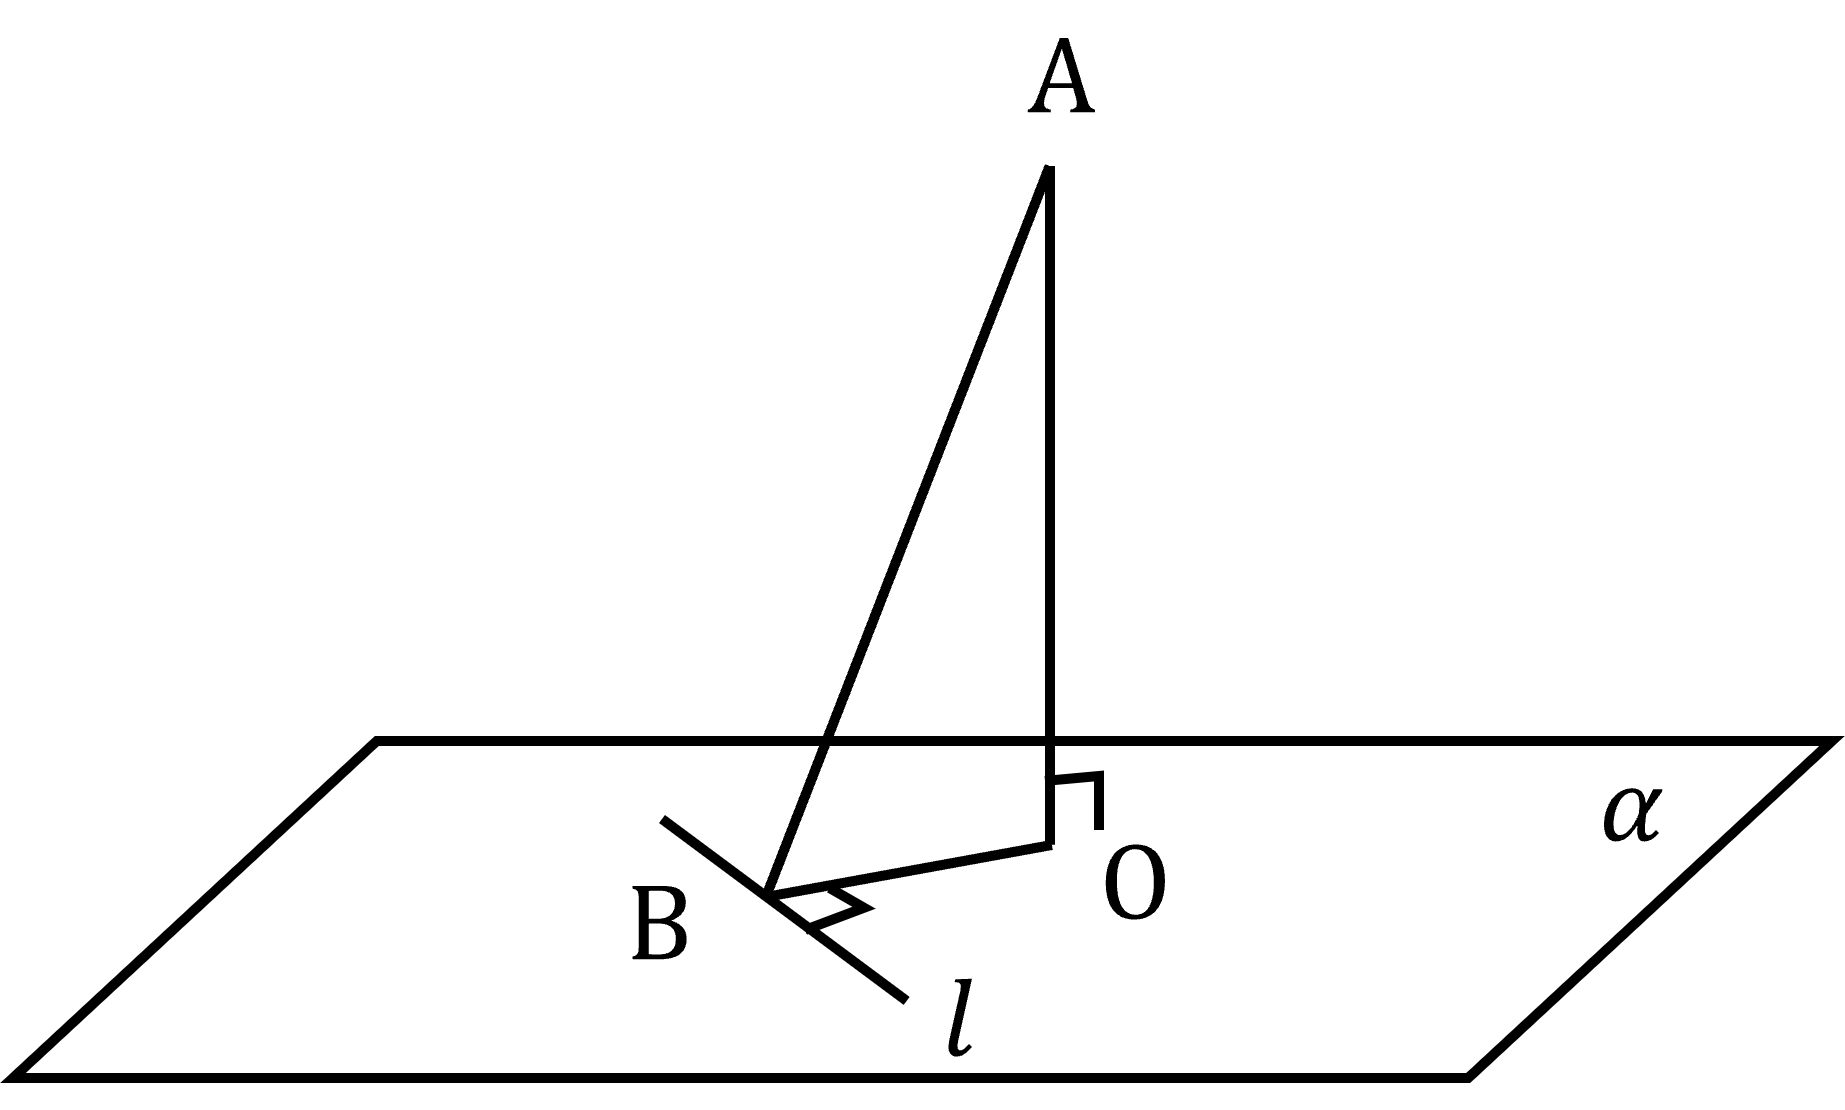
\includegraphics[width=50mm]{fig/10.png}
        \end{center}
    \end{figure}
\end{frame}
%---------------------------------------------------------------
\begin{frame}{空間における直線や平面の位置関係}
    %! 
    \begin{itemize}
        \item 平行な2直線の一方に垂直な直線は他方にも垂直である
        \item 直線$l$が平面$\alpha$上の交わる2直線$m$, $n$に垂直ならば直線$l$は平面$\alpha$に垂直である
        \item 平面$\alpha$の1つの垂線を含む平面は$\alpha$に垂直である
    \end{itemize}
\end{frame}
%---------------------------------------------------------------
\begin{frame}{正多面体の定義}
    %! 
    次の2つの条件を満たす凸多面体を正多面体という
    \begin{itemize}
        \item 各面はすべて合同な多角形である
        \item 各面はすべて合同な多角形であり, 各頂点に集まる面の数は等しい
    \end{itemize}
\end{frame}
%---------------------------------------------------------------
\begin{frame}{オイラー多面体定理}
    %! 
    凸多面体において $v$: 頂点数, $e$: 辺の数, $f$: 面の数
    \begin{eqnarray*}
        v-e+f=2
    \end{eqnarray*}
\end{frame}
%---------------------------------------------------------------
\begin{frame}{倍数の判定法}
    %! 
    \begin{itemize}
        \item 2の倍数: 一の位が0, 2, 4, 6, 8
        \item 5の倍数: 一の位が0, 5
        \item 4の倍数: 下2桁が4の倍数
        \item 3の倍数: 各位の和が3の倍数
        \item 9の倍数: 各位の数の和が9の倍数
    \end{itemize}
\end{frame}
%---------------------------------------------------------------
\begin{frame}{約数の個数}
    %! 
    自然数$N$の素因数分解が$N=p^aq^br^c\cdots$となるとき, $N$の正の約数の個数は
    \begin{eqnarray*}
        (a+1)(b+1)(c+1)\cdots
    \end{eqnarray*}
\end{frame}
%---------------------------------------------------------------
\begin{frame}{最大公約数, 最小公倍数の性質}
    %! 
    2つの自然数$a$, $b$の最大公約数を$g$, 最小公倍数を$l$とする. $a=ga'$, $b=gb'$とすると
    \begin{enumerate}
        \item $a'$, $b'$は互いに素である
        \item $l=ga'b'=ab'=a'b$
        \item $ab=gl$ 特に $g=1$のとき $ab=l$
    \end{enumerate}
\end{frame}
%---------------------------------------------------------------
\begin{frame}{整数の割り算}
    %! 
    整数$a$と正の整数$b$に対して
    \begin{center}
        $a=bg+r$, $0 \leq r \leq b$
    \end{center}
    を満たす整数$q$と$r$がただ1通りに定まる
\end{frame}
%---------------------------------------------------------------
\begin{frame}{連続する整数の積の性質}
    %! 
    \begin{enumerate}
        \item 連続する2つの整数の積は2の倍数である
        \item 連続する3つの整数の積は6の倍数である
    \end{enumerate}
\end{frame}
%---------------------------------------------------------------
\begin{frame}{余りによる整数の分類 }
    %! 
    $k$ は整数とする
    \begin{enumerate}
        \item $2k$, $2k+1$ (偶数, 奇数)
        \item $3k$, $3k+1$, $3k+2$ (3で割った余りが0, 1, 2)
        \item 一般に$m$が2以上の自然数のとき \par
              $mk, mk+1, mk+2, \cdots , mk+(m-1)$
    \end{enumerate}
\end{frame}
%---------------------------------------------------------------
\begin{frame}{合同式}
    %! 
    $m$は正の整数とする\par
    2つの整数$a$, $b$について, $a-b$が$m$の倍数であるとき, $a$と$b$は$m$を法として合同であるといい, 式で$a \equiv b \;\;\;(\mod m)$として表す
\end{frame}
%---------------------------------------------------------------
\begin{frame}{割り算と最大公約数}
    %! 
    2つの自然数$a$, $b$について, $a$を$b$で割ったときの余りを$r$とすると, $a$と$b$の最大公約数は, $b$と$r$の最大公約数に等しい.
\end{frame}
%---------------------------------------------------------------
\begin{frame}{ユークリッドの互除法}
    %! 
    2つの自然数$a$, $b$の最大公約数を求めるには次の手順を繰り返せばよい
    \begin{enumerate}
        \item $a$を$b$で割ったときの余りを$r$とする.
        \item $r=0\Rightarrow b$ が$a$と$b$の最大公約数 \par
              $r>0 \Rightarrow a$ を$b$, $b$を$r$で置き換えて(1)へ
    \end{enumerate}
\end{frame}
%---------------------------------------------------------------
\begin{frame}{1次不定方程式と整数解}
    %! 
    0でない2つの整数$a$, $b$が互いに素であるならば任意の整数$c$について$ax+by=c$を満たす$x$, $y$が存在する
\end{frame}
%---------------------------------------------------------------
\begin{frame}{有限小数, 循環小数の判定法}
    %! 
    既約分数$\frac{m}{n}$において次のことが成り立つ
    \begin{itemize}
        \item 分母$n$の素因数は2, 5だけからなる \par
              $\Leftrightarrow \frac{m}{n}$は有限小数で表される.
        \item  分母$n$の素因数について2, 5以外のものがある \par
              $\Leftrightarrow \frac{m}{n}$は循環小数で表される
    \end{itemize}
\end{frame}
%---------------------------------------------------------------
\begin{frame}{$n$進法, $n$進数}
    %! 
    位置取りの基礎を$n$として数を表す方法を$n$進法といい,\par $n$進法で表された数を$n$進数という
\end{frame}
\end{document}
